
%%%%%%%%%%%%%%%%%%%%%%%%%%%%%%%%%%%%%%%%%%%%%%%%%%%%%%%%%%%%%%%%%%%%%%%%%%%%%%%
%%%%%%%%%%%%%%%%%%%%%%%%%%%%%%%%%%%%%%%%%%%%%%%%%%%%%%%%%%%%%%%%%%%%%%%%%%%%%%%
%%%%%%%%%%%%%%%%%%%%%%%%%%%%%%%%%%%%%%%%%%%%%%%%%%%%%%%%%%%%%%%%%%%%%%%%%%%%%%%
\section{Results} %-----------------------------------------------------------%
\subsection{Evaluation Platform} %--------------------------------------------%
All results were obtained by either interrogating the daemon[s] directly
to inspect their state or by running queries against the SOSflow
databases.
%, such as the one in Figure~\ref{example_query}.
%

%\begin{figure}[h]
%  \centering
%  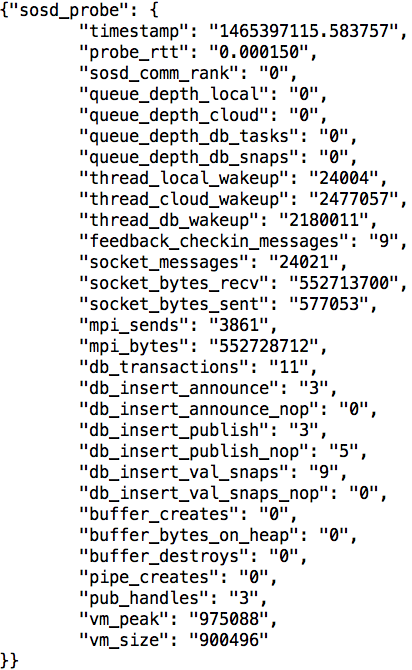
\includegraphics[width=\columnwidth]{images/probe_json_example.png}
%  \caption{JSON Object Returned by SOS's Probe Tool}
%  \label{probe_json}
%\end{figure}
%
%
%


\subsection{Experiment Setup} %-----------------------------------------------%
%
The experiments performed had the following purposes:
%
\begin{itemize}
  %
\item \textbf{Validation} : Demonstrate that the SOSflow model works
  for a general case.
%
\item \textbf{Exploration} : Study the latency and overhead of
  SOSflow's current research implementation.
%
\end {itemize}
%
The SOSflow implementation is general-purpose and we did not need to
tailor it to the deployment environment.
%
The same SOSflow code base was used for each of the experiments.
%
The study was conducted on three machines, the details of which are
given below ---
%
\begin{enumerate}
%
\item \textbf{ACISS} : The University of Oregon's 128-node compute
  cluster.
%
Each node has 72 GB of memory and 2x Intel X5650 2.66 GHz 6-core CPUs,
providing 12 cores per node.
%
Each node is connected together with a 10GigE ethernet switch.
%
%
\item \textbf{Cori} : A Cray XC40 supercomputer at the National Energy Research Scientific
  Computing Center (NERSC).
%
Nodes are equipped with 128 GB of memory and 2x Intel Xeon
E5-2698v3 2.30 GHz 16-core CPUs.
%
Cori nodes are connected by a Cray Aries network with Dragonfly
topology, that has 5.625 TB/s global bandwidth.
%
%
\item \textbf{Catalyst} : A Cray CS300 supercomputer at Lawrence
  Livermore National Laboratory (LLNL).
%
Each of the 324 nodes is outfitted with 128 GB of memory and 2x Intel
Xeon E5-2695v2 2.40 GHz 12-core CPUs.
%
Catalyst nodes transport data to each other using a QLogic InfiniBand
QDR interconnect.
%
\end{enumerate}
%
%
We simulated workflows using the following --- 
%
\begin{enumerate}
%
\item \textbf{LULESH with TAU} : An SOSflow-enabled branch of the
  Tuning and Analysis Utilities program (TAUflow) was created as a
  part of the SOSflow development work.
%
On Cori, TAUflow was used to instrument the Livermore Unstructured
Lagrangian Explicit Shock Hydrodynamics (LULESH) code.
%
During the execution of LULESH, a thread in TAUflow would periodically
awaken and submit all of TAU's observed performance metrics into the
SOSflow system.
%
\item \textbf{Synthetic Workflow} : Synthetic parallel MPI
  applications were developed that create example workloads for the
  SOSflow system by publishing values through the API at configurable
  sizes and rates of injection.
%
\end{enumerate}
%
%


\subsection{Evaluation of SOS Model} %-------------------------------------%
This experiment was performed to validate the SOS Model and
demonstrate its applicability for the general case of workflow
observation.
%
The Cori supercomputer was used to execute a LULESH + TAUflow simulation. 
%
Power and memory usage metrics were collected and stored in SOSflow for
each node.
%
During the execution of the workflow, a visualization application was
launched from outside of the job allocation which connected to
SOSflow's online database and was able to query and display graphs of
the metrics that SOSflow had gathered.
%
\par
%
The LULESH job was run both with and without the presence of SOSflow
(all other settings being equal) in order to validate the ability of
SOSflow to meet its design goals while being minimally invasive.
%
%


\subsection{Evaluation of Latency} %---------------------------------------%
Experiments were performed to study the latency of data moving
through SOSflow.
%
When a value is published from a client into the SOSflow runtime,
it enters an asynchronous queue scheme for both database injection
and off-node transport to an aggregation target.
%
Latency in this context refers to the amount of time that a value
spends in these queues before becoming available for query by
analytics modules.
%
To study latency we ran experiments on both ACISS and Catalyst.
% 
\par
%
Tests run on ACISS were
deployed with the Torque job scheduler as MPICH2 MPI applications at
scales ranging from 3 to 24 nodes, serving 10 Synthetic Workflow processes per node in all cases.
%
The ACISS battery of runs were tuned as stress tests to ensure that
the sosd daemons could operate under reasonably heavy loads.
%
In the 24-node ACISS experiment (Figure~\ref{aciss_lat_24_agg}),
SOSflow clients published 72,000,000 double-precision floats
with associated metadata during a 90 second window containing three
rounds of extremely dense API calls.
%
\par
%
Latency tests were performed on LLNL's Catalyst machine at
various scales up to 128 nodes, with 8 data sources contributing
concurrently on each node in each case.
%
Catalyst's tests measured the latency introduced by sweeping across three
different parameters:
\begin{itemize}
\item Count of unique values per publish
\item Number of publish operations per iteration
\item Delay between calls to the publish API
\end{itemize}
%
Unlike the ACISS experiments, the Catalyst tests did not attempt to
flood the system with data, but rather aimed to observe how slight
adjustments in size and rates of value injection would impact the
latency of those values.
%
%




\subsection{Results} %--------------------------------------------------------%
%
%
\subsubsection{SOS Model Validation} %----------------------------------------%
%
SOSflow was able to efficiently process detailed performance
information from multiple sources on each node.
%
During the LULESH run, SOSflow's online database successfully serviced
queries on-line, and the results were plotted as an animated live
view of the performance of the workflow.
%
\begin{figure}[h]
\centering
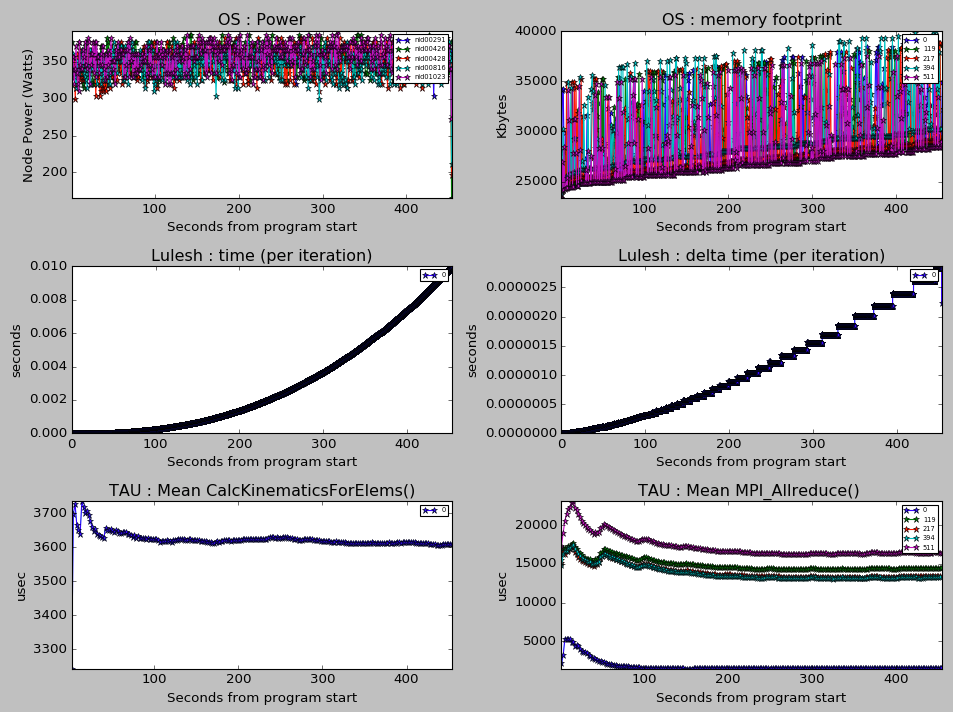
\includegraphics[width=\columnwidth]{images/512_procs.png}
\caption{On-line Workflow Performance Visualization Using SOSflow on
  Cori.  Live View of 512 Processes From Three Perspectives: OS,
  LULESH, TAU}
\label{cori_visualization}
\end{figure}
%%%%%
%
The cost of using SOSflow was calculated simply as the increase in
walltime for LULESH + SOSflow, expressed as a percentage of the walltime
of LULESH by itself.
%
The results of these runs are shown in Figure~\ref{cori_results}.
%
\begin{figure}[h]
\centering
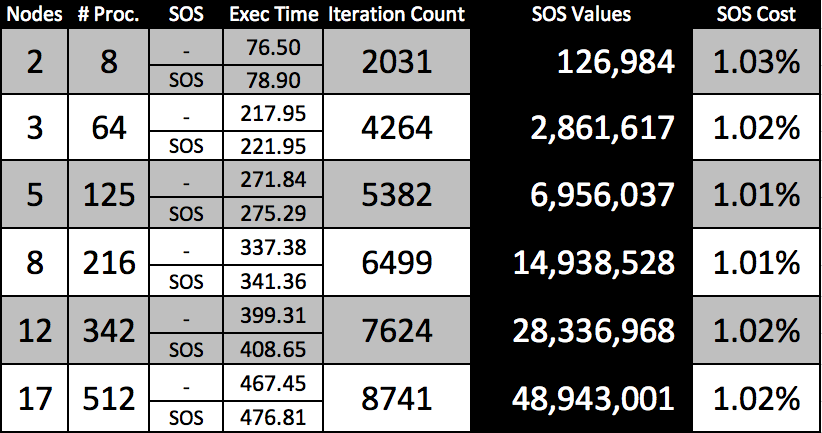
\includegraphics[width=\columnwidth]{images/cori_results.png}
\caption{Percent Increase in LULESH Running Time When SOSflow is Used}
\label{cori_results}
\end{figure}
%
%
\subsubsection{Evaluation of Latency} %-------------------------%
%
The on-node (Figure~\ref{catalyst_avg_node}) and aggregate
(Figure~\ref{catalyst_avg_128}) results from the largest 128-node runs
are presented here.
%
Results from smaller runs are omitted for space, as they show nothing
new: ``Time in flight'' queue latency at smaller scales linearly
approached the injection latency figures for a single (on-node)
database.
%
\par
%
In the 128-node runs, across all configurations, the mean latency
observed was ~0.3 seconds (and a maximum of 0.7 seconds) for a value,
and its full complement of metadata and timestamps, to migrate from
one of 1,024 processes to the off-node aggregate data store, passing
through multiple asynchronous queues and messaging systems on 128
nodes.
%

%%%%%
\begin{figure}[h]
\centering
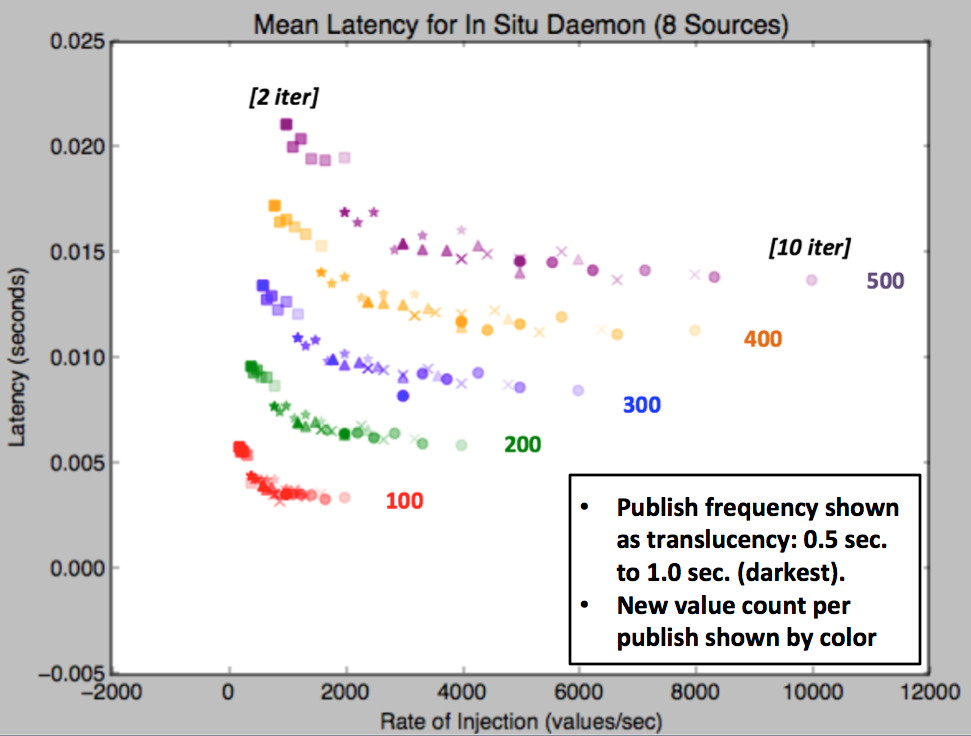
\includegraphics[width=\columnwidth]{images/avg_node.png}
\caption{Average Latency for In Situ Database (128 nodes on Catalyst)}
\label{catalyst_avg_node}
\end{figure}
%%%%%

%%%%%
\begin{figure}[h]
\centering
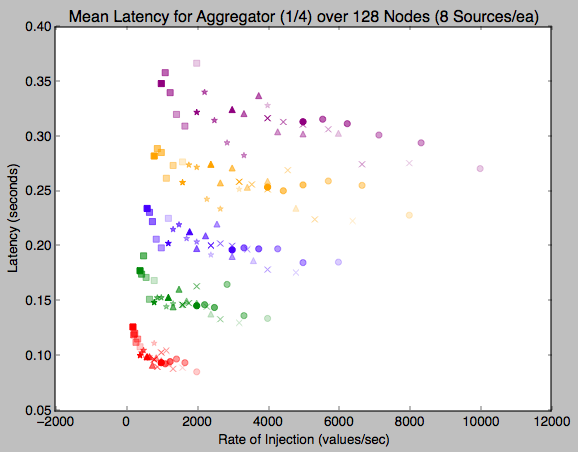
\includegraphics[width=\columnwidth]{images/avg_128.png}
\caption{Average Latency for Aggregate Database (128 nodes on Catalyst)}
\label{catalyst_avg_128}
\end{figure}
%%%%%

%
The in situ and aggregate results in Figures ~\ref{catalyst_avg_node}
and Figure~\ref{catalyst_avg_128} are promising, given the research
version of SOSflow being profiled is not optimized.
%
Exploring the optimal configuration and utilization of SOSflow is left
to future research effort.
%
\subsection{Discussion}
%
Many of the behavioral characteristics of SOSflow are the product of
its internal parameters and the configuration of its runtime
deployment, rather than products of its data model and algorithms.
%
For now, the effort was made to select reasonable default SOSflow
configuration parameters and typical/non-priviledged cluster queues
and topologies.
%
Because of the general novelty of the architecture, the results
presented here could be considered the \textit{performance baseline}
for SOSflow to improve on as the research matures.
%
\par
%
Expanding on the direct experimental results, here are some additional
experiences and observations about the behavior of SOSflow: ---
%
\subsubsection{Aggregation Topology}
%%%%%
The current version of SOSflow is configured at launch with a set
number of aggregator databases.
%
The validation tests on ACISS used 3 sosd\_db instances to divide up
the workload, while the TAUflow + LULESH experiments on Cori used a
single aggregator.
%
The parameter sweeps run on the LLNL Catalyst machine were done with
four sosd\_db aggregation targets at 128 nodes.
%
Tests on ACISS and Catalyst were exploring the latency of data
movement through SOSflow, and so both configurations featured
dedicated nodes for sosd\_db aggregators to avoid contention
with other on-node work.
%
The Cori runs captured a real application's behavior, and was primarily
intended to demonstrate the fitness of SOSflow for capturing the
performance of a scientific workflow along with meaningful context.
%
Instances of aggregators can be spawned, as many as needed, in order
to support the quantity of data being injected from a global
perspective.
%
All data sent to SOSflow is tagged with a guid.
%
This allows for shards of the global information space to be concatenated
after the run concludes without collision of identities wiping out
distinct references.
%
\par
%
The data handling design trade-offs made for SOSflow do not prioritize
the minimization of latency, but focus rather on gracefully
handling spikes in traffic by growing (and then shrinking) the space
inside the asynchronous message queues.
%
After a value is passed to SOSflow, it is guaranteed to find its
way into the queryable data stores, and there are timestamps attached
to it that capture the moment it was packaged into a publication handle in
the client library, the moment it was published to the daemon, and
even the moment it was finally spooled out into the database.
%
Once it is in the database, it is trivial to correlate values
together based on the moment of their creation, no matter
how long the value was sequestered in the asynchronous queues.
%
\par
%
During the ACISS stress-tests, values were injected into the
SOSflow system faster than they could be spooled from the queues into
the database.
%
While every value will eventually be processed and injected into the data
store, some values wound up having to wait longer than others as the queue
depth increased.
%
The asynchronous queues have thread-sequential FIFO ordering, but
because the MPI messages are queued up based on their arrival time,
and a batch is handled completely before the next is processed, there
is no real-time interleaving of database value injections, they are
injected in batches.
%
Near the bottom of the pile of MPI messages, the latency continually
increases until that batch is injected.
%The latency for values in the batches near the bottom of the pile of
%MPI messages consistently increases until their batch is injected.
%
This accounts for the observed saw-tooth pattern of increasing latency
seen in Figure~\ref{aciss_lat_24_agg}, which is not seen in
Figure~\ref{aciss_lat_24_situ}.
%
%


%%%%%
%\begin{figure}[h]
%\centering
%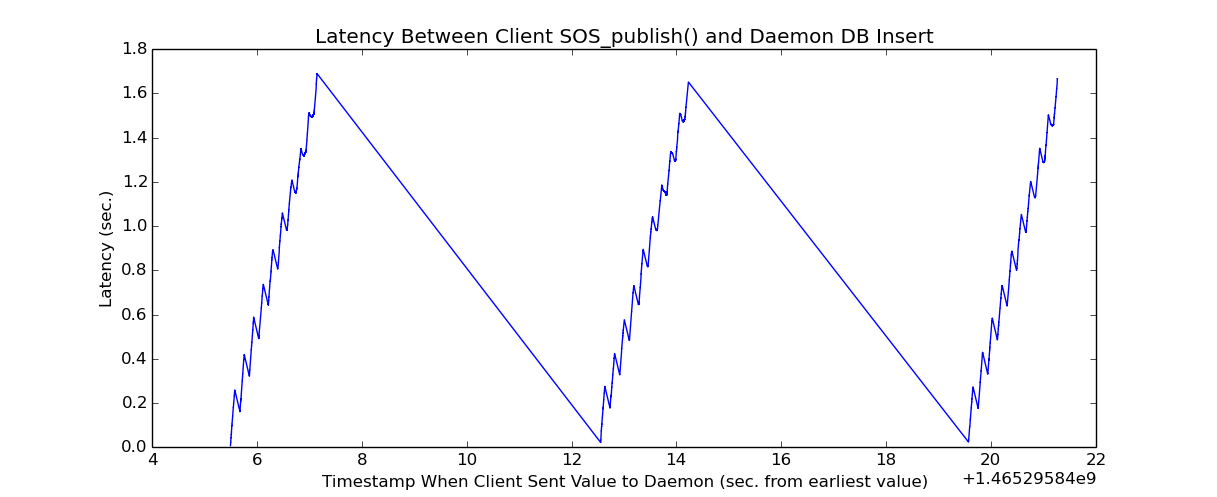
\includegraphics[width=\columnwidth]{images/aciss_latency_3_situ.png}
%\caption{In Situ Latency (3 Nodes, 30 Applications)}
%\label{aciss_lat_3_situ}
%\end{figure}
%%%%%

%%%%%
%\begin{figure}[h]
%\centering
%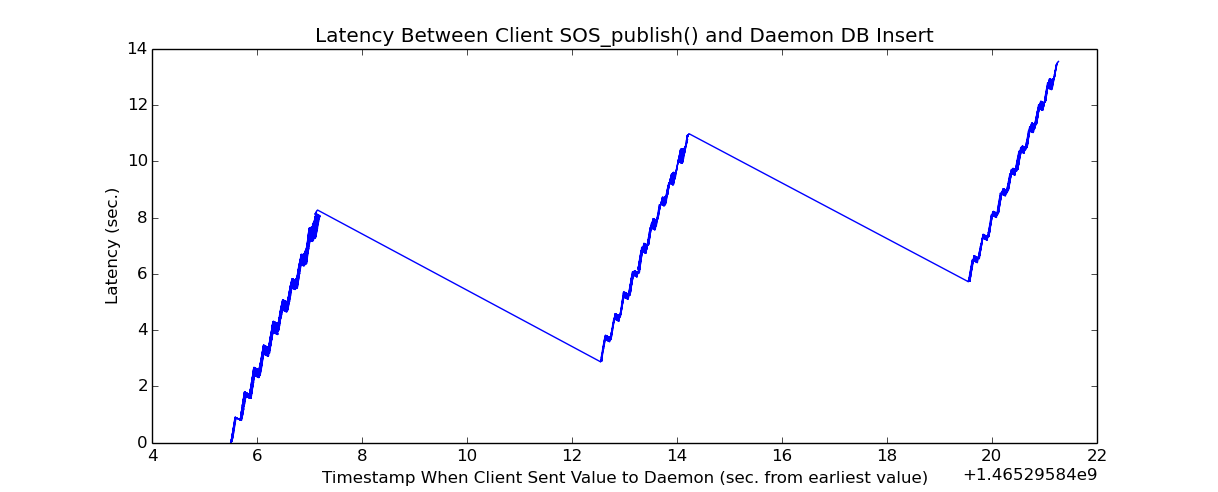
\includegraphics[width=\columnwidth]{images/aciss_latency_3_agg.png}
%\caption{Aggregate sosd(db) Latency (3 Nodes, 30 Applications)}
%\label{aciss_lat_3_agg}
%\end{figure}
%%%%%

%%%%%
%\begin{figure}[h]
%\centering
%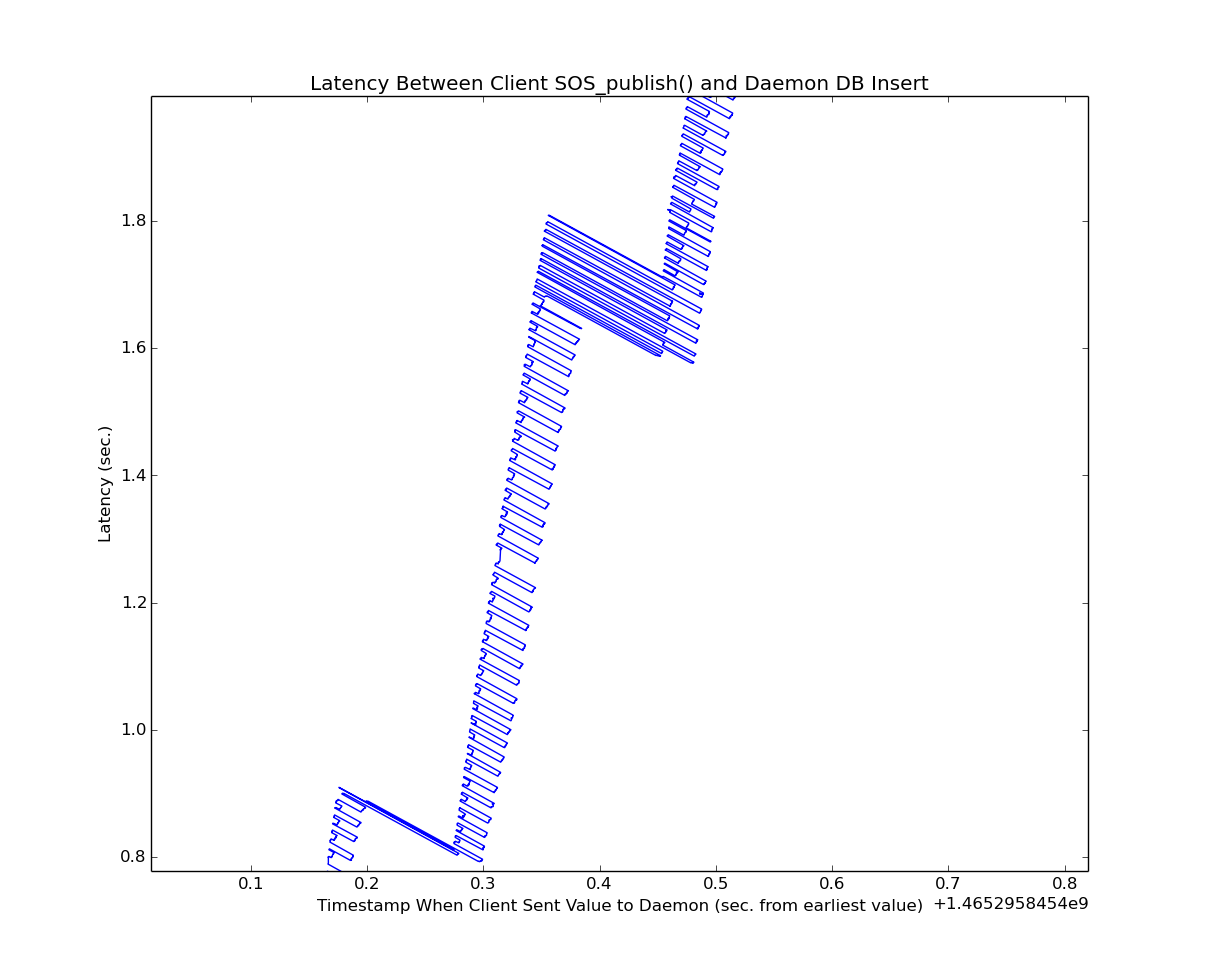
\includegraphics[width=\columnwidth]{images/aciss_latency_3_agg_zm.png}
%\caption{Aggregate sosd(db) Detail (3 Nodes, 30 Applications)}
%\label{aciss_lat_3_agg_detail}
%\end{figure}
%%%%%

%%%%%
\begin{figure}[h]
\centering
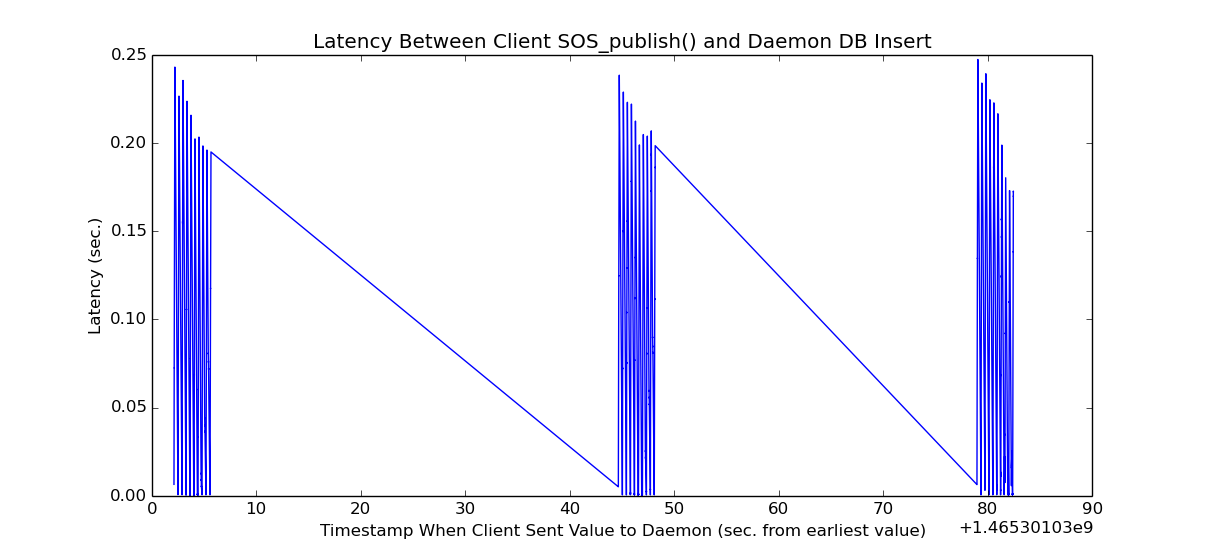
\includegraphics[width=\columnwidth]{images/aciss_latency_24_situ.png}
\caption{In Situ Latency (24 nodes on ACISS, 240 Applications)}
\label{aciss_lat_24_situ}
\end{figure}
%%%%%

%%%%%
\begin{figure}[h]
\centering
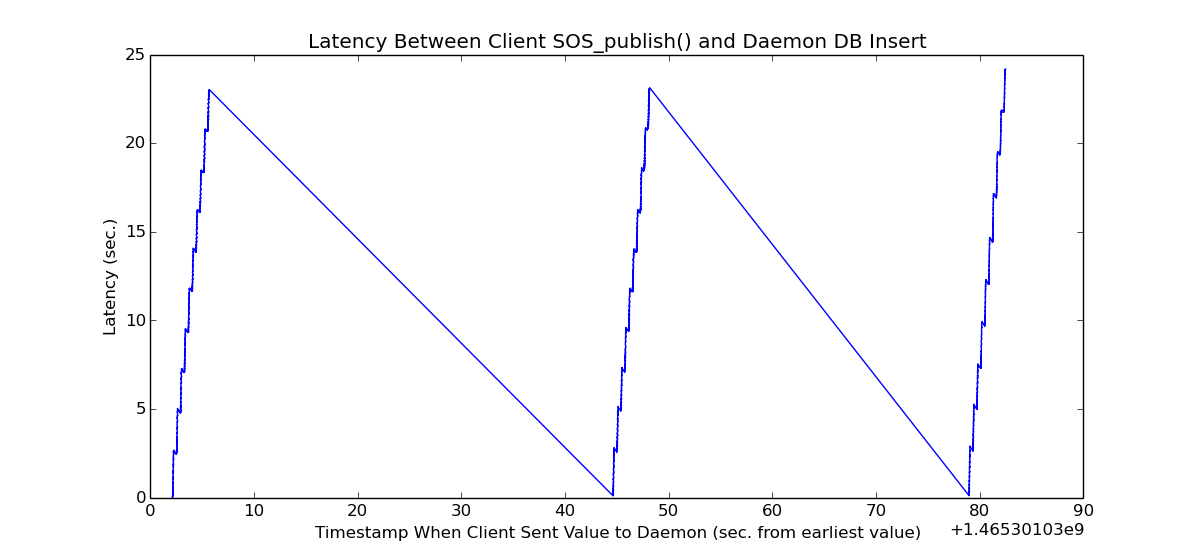
\includegraphics[width=\columnwidth]{images/aciss_latency_24_agg.png}
\caption{Aggregate Latency (24 nodes on ACISS, 240 Applications)}
\label{aciss_lat_24_agg}
\end{figure}
%%%%%
%
\par
%
%

\subsubsection{Time Cost of Publish API} %-----------------------------------%
%
As an accessory to the study of value latency, the length of time that
a client application will block inside of an SOSflow API routine was
also evaluated.
%
In situ interactions between libsos routines and the daemon are
nearly constant time operations regardless of the daemon's workload.
%
Care was taken in the daemon's programming to prioritize rate of message
ingestion over immediacy of message processing so that SOSflow API calls
would not incur onerous delays for application and tool developers.
%
The constancy of message processing speed is shown in
figures~\ref{sock_cost} and \ref{sock_cost_detail}, where the round
trip time (RTT) of a probe message between a client and the daemon
(blue) is projected over a graph of the number of new messages
arriving in a sample window (red).
%
\par
%
This information was gathered by sending 9000+ probe messages over a 15
minute window, with a single sosd\_listener rank processing an average
of 724 client messages a second in total, arriving from four different
processes on an 8-way Xeon node.
%
The messages from SOS clients contained more than 14.7 GB of data,
averaging to 338kB per message.
%
Though there are a few spikes in the probe message RTT visible in
Figure~\ref{sock_cost}, they are likely not related to SOSflow at all,
as Figure~\ref{sock_cost_detail} reveals in detail.
%
The RTT holds steady during low and high volume of traffic from the
other in situ client processes.
%
The mean RTT for the probe messages was 0.003 seconds, and the maximum
RTT was 0.07 seconds.
%
%%%%%
\begin{figure}[h]
\centering
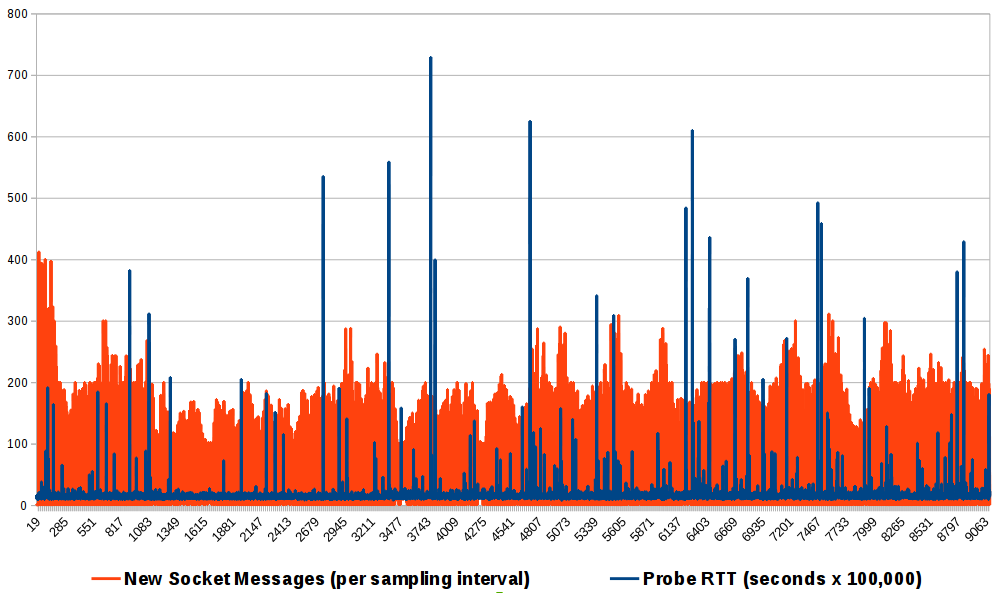
\includegraphics[width=\columnwidth]{images/icebox_api_cost_when_slam.png}
\caption{SOSflow Socket Communication Cost, Projected Over Message Count}
\label{sock_cost}
\end{figure}
%%%%%

%%%%%
\begin{figure}[h]
\centering
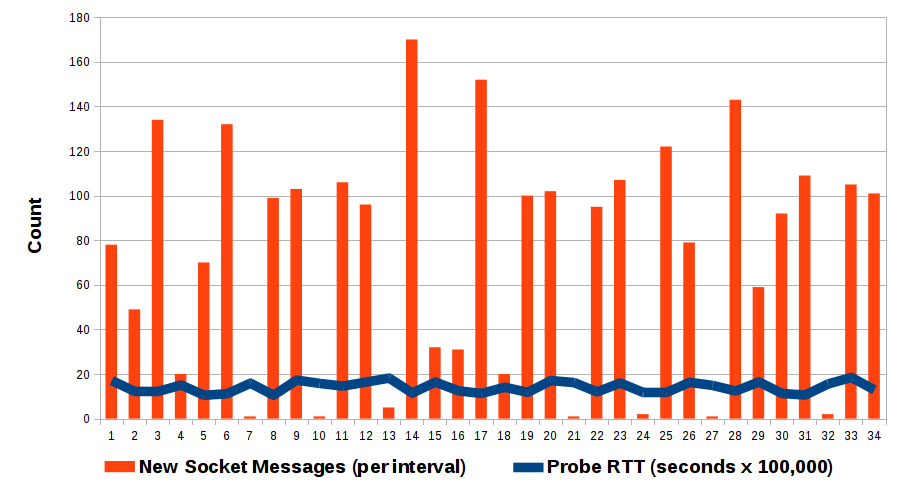
\includegraphics[width=\columnwidth]{images/icebox_api_cost_zoom.png}
\caption{SOSflow Socket Communication Cost (Detail)}
\label{sock_cost_detail}
\end{figure}
%%%%%
%
\par
%
These results show that the cost of making SOSflow API calls is
relatively low, and holds constant under changing sosd\_listener
workload.
%
%





%%%
%%%  EOF
%%%
